\documentclass[a4paper,11pt]{article}

% set up sensible margins (same as for cssethesis)
\usepackage[paper=a4paper,left=30mm,width=150mm,top=25mm,bottom=25mm]{geometry}
\usepackage{setspace}               % This is used in the title page
\usepackage{graphicx}               % This is used to load the crest in the title page
\usepackage{poltakmacros}           % Personal macros included in file 'poltakmacros.sty'
\usepackage{enumitem}               % For nested enum lists
\edef\restoreparindent{\parindent=\the\parindent\relax}
\usepackage{parskip}
\restoreparindent
\usepackage{pdflscape}
\usepackage[table]{xcolor}
\usepackage{colortbl}
\usepackage{float}
\usepackage[hidelinks]{hyperref}
\usepackage{url}
\usepackage[font={small}]{caption}
\usepackage[hidelinks]{hyperref}
\usepackage{import}

\begin{document}

% Cover page + TOC
% Set up a title page
\thispagestyle{empty} % no page number on very first page
% Use roman numerals for page numbers initially
\renewcommand{\thepage}{\roman{page}}

\author{Jonathan Poltak Samosir}
\title{Honours Thesis}

\begin{spacing}{1.5}
\begin{center}
{\Large \bfseries
Clayton School of Information Technology\\
Monash University}

\vspace*{30mm}


\includegraphics[width=5cm]{img/MonashCrest.pdf}

\vspace*{15mm}

{\large \bfseries
Honours Thesis --- Semester 1, 2015
}

\vspace*{10mm}

{\LARGE \bfseries
A study of data stream processing systems for use with railway
}

\vspace*{20mm}

{\large \bfseries
Jonathan Poltak Samosir

[2271 3603]

\vspace*{20mm}

Supervisors: \parbox[t]{50mm}{\mbox{Dr Maria Indrawan-Santiago}\\Dr Pari Delir Haghighi}
}

\end{center}
\end{spacing}

\newpage


\tableofcontents

\newpage
% Now reset page number counter,and switch to arabic numerals for remaining page numbers
\setcounter{page}{1}
\renewcommand{\thepage}{\arabic{page}}



% Abstract
\section{Abstract}
\label{sec:abstract}
%!TEX root = thesis.tex
\section*{Abstract}
\label{sec:abstract}



% Section 1: Intro/proposal
\section{Introduction}
\label{sec:intro}
%!TEX root = thesis.tex
% Start of content
\chapter{Introduction}
\label{sec:intro}

Currently, as a society, we are generating very large amounts of data from a large range of different sources. These
sources include scientific experiments, such as the Australian Synchrotron~\cite{web:synchrotron} and The Large Hadron
Collider~\cite{web:LHC}, companies, such as Amazon~\cite{web:Amazon}, and also data generated by end users of products,
such as social networks. The rate of data that is being generated is constantly increasing, presenting major challenges
when it comes to the storage and processing of that data~\cite{bohlouli_towards_2013}. This is what is often referred to
now as ``Big Data''. A further big data project, that will be looked into as the basis of the project outlined in this
thesis, is the automated monitoring of railway tracks and cars by the Institute of Railway Technology at Monash University
(IRT)~\cite{web:monash_irt}.

Out of all of these data that we are faced with in such projects, often only specific parts of the data are of particular use for given
purposes. Hence, rather than attempting to store all the new data that is being generated, an increasingly popular method of
dealing with such data, in both academia and industry associated with big data, is the processing and analysis of
data in realtime as it is received. This is also known as online processing, or single pass processing, where data is
processed in real time before being discarded. Further options also exist where data is stored after processing, depending
on the specific use-case.

There are currently numerous realtime data processing systems that are in development and in production use, both in
industry and academia. Examples of these realtime data processing frameworks include the widely used Storm
project~\cite{web:Storm}, developed at BackType and Twitter, Inc., and also the up-and-coming Spark Streaming
project~\cite{web:SparkStreaming}, developed at UC Berkeley's AMPLab~\cite{web:UCBerkelyAMCLab}, both of which are
open-source projects. While there are a growing number of these projects being developed, often these projects are designed
with a particular type of processing in mind. For example, the before
mentioned Spark Streaming project, along with its mother project, Spark~\cite{web:Spark}, was originally designed for highly
parallelisable data with the use-case in mind of processing data in-memory using highly iterative machine learning
algorithms related to data analytics~\cite{liu_survey_2014}.

What is proposed in this chapter is a realtime big data processing pipeline for the aforementioned railway monitoring
system by the IRT at Monash University. This processing pipeline will allow the possibility that data is able to be
streamed in realtime from the railway, and processed according to the team's given processing requirements. Multiple
technologies exist in which this pipeline can be implemented, so a technology recommendation will be formed through
the testing and evaluation of different implementations in different technologies.

This chapter will be structured as follows:\\
A brief outline of the big data processing domain, both batch and realtime processing, will be given
in~\sectref{sec:research_context}. Furthermore, an overview of the Monash University Institute of Railway Technology's
project, upon which this project is based on, will be covered in the aforementioned section. In~\sectref{sec:objectives},
the aims of the entire project will be given, as well as more specific goals and aims relating to the sub-project
covered in this thesis. Research questions for this sub-project will be given in~\sectref{sub:research_questions}.
Finally, the structure of this overall thesis will be given in~\sectref{sub:proposed_thesis_chapter_headings}, before
concluding this chapter in~\sectref{sec:summary}.

% section introduction (end)



\section{Research Context} % (fold)
\label{sec:research_context}

\subsection{Big Data} % (fold)
\label{sub:big_data}

Big data, as explained previously, is becoming commonplace in both industry and academia. Everyday companies are finding
that they are generating large volumes of data and that their traditional relational database management system (RDMBS) solutions cannot
scale to the epic proportions needed to handle this data in an efficient and robust manner~\cite{marz2013principles}.
Hence, companies and academics alike have started looking at alternative solutions designed with the goal of handling
these massive datasets.

The most popular solution for this problem, up until recently, has been the MapReduce % TODO: Add reference to MR
 model of programming along with
some type of scalable distributed storage system~\cite{bifet_mining_2013}. The MapReduce model was started at Google,
Inc.\@ with their own proprietary implementation along with their proprietary distributed file system, known as the Google
File System (GFS)~\cite{ghemawat_google_2003}. Without going into the low-level details of MapReduce and GFS, the use of this solution at Google
allowed the company to easily handle all the data that was coming into their servers, including those related to Google Search, and perform the necessary
processing operations that was needed at the time~\cite{ghemawat_google_2003,dean_mapreduce:_2008}.

% subsection big_data (end)

\subsection{Batch Data Processing} % (fold)
\label{sub:apache hadoop}

From the success of MapReduce usage combined with GFS, at Google, the open-source community responded swiftly with the
development of the Apache Hadoop framework\footnote{https://hadoop.apache.org}. Hadoop originally offered an open-source
implementation of MapReduce and their own open-source distributed file system known as the Hadoop Distributed File System
(HDFS)~\cite{shvachko_hadoop_2010}.

Hadoop soon became the subject of mass-adoption in both industry and academia, being deployed at a fast rate.
Development of the Hadoop framework also grew at a fast rate, with new applications related to HDFS and MapReduce being
built on top of Hadoop, greatly benefiting the ecosystem as a whole. Some of these applications grew into widely adopted
systems in their own right. For example, Hadoop applications such as Apache Pig~\cite{gates2009building} and
Hive~\cite{thusoo2010hive} allow for easy querying and manipulation of data stored on HDFS, both coming with the
addition of their own query languages~\cite{olston_pig_2008}.

As further non-MapReduce model applications became of interest to the Hadoop community, Hadoop soon
developed a further abstraction on top of the underlying resources (in most cases, HDFS). The goal of this was to
facilitate the development and deployment of many different applications, varying in use-case, which could be run on the
Hadoop ecosystem, without forcing developers to fit their application into the MapReduce model. This development was
known as Apache Hadoop YARN:\@ Yet Another Resource Negotiator, which can be thought of as an operating system-like abstraction sitting
atop of the available Hadoop resources~\cite{vavilapalli_apache_2013}. The abstraction provided by YARN facilitated the
development of much more advanced, and non-MapReduce technologies which have since become widely used parts of the
Hadoop ecosystem~\cite{harrison_hadoops_2012}.

% subsection apache_hadoop (end)

\subsection{Realtime Data Processing} % (fold)
\label{sub:prop_realtime_data_processing}

One of the major limitations of Hadoop, and the MapReduce model in general, soon became obvious:\@ MapReduce was designed
with the goal of being able to process batches of data, hence, given Hadoop's dominance, batched data processing was the
focal point of the entire distributed data processing domain~\cite{kamburugamuve_survey_2014}. Essentially, batched data
processing is where data gets collected first into large enough batches before being processed all-at-once. The point of
processing in such a way is so there would be less overheads than attempting to process each individual datum as it
arrives. For a lot of use-cases this was, and still is, fine as there were no other drawbacks apart from a high level of
latency between the stages of when the data arrives and when it gets processed. However, for other applications, such as
stock trading, sensor monitoring, and web traffic processing, a more low-latency, realtime solution was
needed~\cite{kamburugamuve_survey_2014}.

Soon, many solutions, with different use-cases and design goals, were developed in the area of distributed stream
processing systems (DSPS). Given the Hadoop ecosystem that was already widely adopted, most of these DSPSs were built
upon the still new YARN layer, ensuring overall compatibility with the Hadoop ecosystem, and the underlying HDFS. Some
examples of such projects include the beforementioned Apache Storm, currently being used at Twitter,
Inc.~\cite{toshniwal_stormtwitter_2014}, among many other companies. Also up-and-coming projects, such as Apache Samza
which is a recently open-sourced project, currently being used in production at LinkedIn Corporation~\cite{web:Samza}.

% subsection realtime_data_processing (end)

\subsection{Monash IRT Railway Project} % (fold)
\label{sub:monash_irt_railway_project}

The railway project that has been developed at Monash University's Institute of Railway Technology\footnote{https://platforms.monash.edu/irt/}
uses numerous sensor
technologies on certain train cars, such as the Track Geometry Recording Car (TGRC) and the Instrumented Ore Car (IOC),
to monitor railway track conditions and detect track abnormalities~\cite{darby2003development,darby2005track}.
These train cars operate in the Pilbara region of Western Australia, continuously performing round trips from a port
to a given loading point, where they are loaded with recently mined minerals and ores.

As is currently the case, data is received and processed using batch data processing technologies. Due to limited coverage
of cellular networks in the Pilbara region of Western Australia, in which the trains currently operate, sensor data from
a given trip is automatically transmitted in large batches to be received by remote servers once a train has concluded a
round trip and
arrives back in port from a loading point~\cite{thomas2012taking}. Given the current cellular network infrastructure in
the region, this is the only feasible option for transmission of data, however Monash IRT have indicated that given
future improvements in cellular network infrastructure, streaming the data back to remote servers in realtime is a likely
possibility. This leads to the potential possibility of this research project's outcomes outlined in this thesis.

The form of batch handling and processing performed on the railway data currently leads to a number of limitations and
problems. The data is currently stored in a relational database management system (RDBMS), and with the current
implementation
of the sensors, the data received is not consistently structured. In fact, the only sensor data guaranteed to be received
in each batch is geographic location and time. Due to the highly structured nature of RDBMS technology, certain work-arounds
need to be performed on the data so that it is compliant to RDBMS schemas, such as the insertions of default values in
the case of missing attributes. Furthermore, low query performance has been noted as a problem plaguing the IRT team
working with the railway data. They wish to resolve these problems by looking into non-relational models for their data
storage and processing systems.

% subsection monash_irt_railway_project (end)

% section research_context (end)



\section{Research Aim} % (fold)
\label{sec:objectives}

The main aim of the entire IRT research project is to develop a fully automated, non-relational big data pipeline to manage
the data received from railway car sensors as a part of Monash University's Institute of Railway Technology project. The
intention is to replace their current relational solution, with a non-relational big data system, offering at least the same capabilities at a larger scale and
with higher performance. The scope of this project is relatively large, and the project, or sub-project, outlined in this
thesis only covers a portion of the greater aforementioned project.

The main aim of this sub-project, outlined in this thesis, is to investigate possible solutions of dealing with the railway sensor data being
streamed and processed in realtime. Based on identified candidate solutions, a recommendation will be formed which will be
used by the IRT team to implement their required realtime processing logic.

To allow the possibility of realtime data streaming from the railway sensors, and forming a recommendation for the most
suitable solution, appropriate data stream processing system
(DSPS) technologies need to be looked at, tested, and evaluated. This makes up the core part of this sub-project's work.
These DSPS technologies need to appropriately take, or accept, the data from some specified source, \eg the sensors, apply
any realtime processing logic that is required, \eg pre-processing, then forward the data on for handling at
another source, \eg long term storage, such as HDFS.

A data filtering ``pipeline'', through which the sensor data flows, will need to be implemented in each of the candidate
DSPS technologies, which can then be used for the testing and evaluation.
By the end of this sub-project, we aim to have proof-of-concept implementations of the pipeline working on the National
eResearch Collaboration Tools and Resources (NeCTAR) cloud services~\cite{web:Nectar}, making use of the candidate DSPS
technologies, along with our overall DSPS technology recommendation for use in the IRT project.

% section objectives (end)



\section{Research Questions} % (fold)
\label{sub:research_questions}

The following research questions are the main focus points of this sub-project:

\begin{enumerate}
  \item\label{item:dsps} Which existing DSPS technologies can be used to build a data filtering pipeline for the Monash
  University IRT project?
  \item\label{item:pipeline} What criteria-based qualitative and performance-based quantitative tests can be performed
  to \textbf{recommend} a particular DSPS technology for building the pipeline?
  \item\label{item:recommendations} Can the data filtering pipeline be designed to be extensible, allowing for the
  addition of future realtime processing requirements?
\end{enumerate}

Additionally, after answering each of these preliminary research questions, we will want to properly implement the
theoretical discoveries from each stage. We do this with the goal of achieving a deployable pipeline that can be then
be used in the testing and overall evaluation stages.

% subsection research_questions (end)


\section{Thesis Structure} % (fold)
\label{sub:proposed_thesis_chapter_headings}

The proposed structure of the remainder of the thesis is as follows. Chapter 2, in~\sectref{sec:litrev}, looks at prior
research and work into the area of big data stream processing, performed both in industry and academia.
A clear overview of the DSPS technologies chosen for this project, along with the design and implementation
of the experimental systems to be used in the evaluation will be given in Chapter 3, in~\sectref{sec:implementation}.
An overview of the testing metrics, environment, results, and an overall evaluation discussion will be given in Chapter 4, in~\sectref{sec:evaluation}.
Finally, Chapter 5, in~\sectref{sec:conclusion} will conclude the thesis, highlighting the contribution made through this research project,
along with highlighting any future work that have been made apparent as the result of this project.

% subsection proposed_thesis_chapter_headings (end)


\section{Summary} % (fold)
\label{sec:summary}

This chapter has introduced the overall project, and in-turn the sub-project upon which this thesis will be based. It
has briefly described the current state of the Monash University Institute of Railway Technology's project and the current
problems that they are faced with, such as the need to deal with non-consistently structured data and low query
performance. These problems are exacerbated given the non-realtime nature of the current data, where issues with sensors
are only discovered much later after-the-fact. To overcome these issues, and to look forward into the hypothetical,
but likely, possibility of having the technological infrastructure to support realtime data processing, this research
aims to develop a realtime processing pipeline, taking the data straight from the railway sensors and perform any
needed realtime processing, and come up with a DSPS technology recommendation for the implementation of this pipeline.

This chapter also outlined a brief context of the research project and big data as a whole, the scope of this sub-project,
and this sub-project's research questions. Finally it was concluded with an overview of the entire structure of this thesis. The
following chapter will look into previous research that has been done on realtime big data processing and handling,
along with going into more detail of the railway project's needs.

% section summary (end)



% Section 2: Lit review
\section{Literature Review}
\label{sec:litrev}
%!TEX root = thesis.tex
% Start of content
\section{Literature Review}
\label{sec:litrev}

The realtime processing of big data is of great importance to both academia and industry. Advancements and progress in
modern society can be directly attributed back to data. The value of data has become more apparent, and data has become
a sort of currency for the information economy~\cite{st2009examining}. Hence, those in society who realised the value of
data early hold immense power over the entire economy, and in turn society, overall~\cite{lievesley1993increasing}.
From seemingly inconsequential gains at the macro level, such as the ability to more
accurately predict the rise and fall of airline tickets~\cite{darlin2006airfares}, to those of utmost importance for
society as a whole, such as predicting and tracking the spread of the Swine Flu Pandemic in 2009 more accurately than
the United States Centers for Disease Control and Prevention could~\cite{ritterman2009using,mayer2013big}. It is
applications of big data processing like these that have been recognised by academics and organisations in
industry alike, with the last decade seeing a major shift in research and development into new methods for the handling
and processing of big data.

This review will give a background on the types and classes of big data, as well as the various methods employed to
process those given classes of data. We will more specifically be focusing on the methods that are involved with the
analysis and processing of realtime data streams, as opposed to the batch processing of big data. This review will look
into detail at previous work that has been done in the field of big data, specifically those works that have had a
greater influence on the field  as a whole. This includes both works looking specifically at the processing of streaming
data, and works involving processed big data in batch mode, given that batch mode processing arguably led onto the
current hot-topic of realtime stream processing.

This review will be structured in two main sections.
In~\sectref{sec:big_data_processing_background}, an overview will be given of the major open-source big data processing
systems in the scope of the Hadoop ecosystem. A special emphasis will be given to realtime data processing systems,
otherwise known as data stream processing systems (DSPSs), given that the main area of this research is focusing on
realtime data processing. This section will also be concluded with a brief comparison of the presented systems.
In~\sectref{sec:conclusion} an analysis and discussion will be given on the content covered from the relevant
literature, as well as identifying how the research contributions of this project will address the gaps found in the
relevant literature.

% section introduction (end)


\subsection{Big data processing background} % (fold)
\label{sec:big_data_processing_background}

Much more work has been done in the area of data processing than the area related to classification of data; both in the
areas of big data and traditional data processing. Unlike data classification, which was more aimed at the classifying
of data in general, when looking at data processing, we are more interested in the relatively newer technologies which
enable the processing of big data, both in batch mode and realtime. Note that in this review, we will refer to the
processing of data in realtime as simply ``realtime data processing''. This term should be assumed to encompass the
meaning that is also often represented as ``data stream processing'', ``realtime stream processing'', and ``stream
processing''.

\subsubsection{Batch data processing} % (fold)
\label{sub:batch_data_processing}

Over the last decade, the main ``go-to'' solution for any sort of processing needed on datasets falling under the
umbrella of big data has been the MapReduce programming model on top of some sort of scalable distributed storage
system~\cite{bifet_mining_2013}. From a very simplified functionality standpoint, the MapReduce programming model essentially
combines the common \textbf{Map} and \textbf{Reduce} functions (among others), found in the standard libraries of many functional
programming languages, such as Haskell~\cite{lammel2008google} or even Java 8~\cite{su2014changing}, to apply a specified
type of processing in a highly parallelised and distributed fashion~\cite{yang2007map}.

The MapReduce data processing model specialises in batch mode processing. Batch data processing can be thought of where
data needed to be processed is first queued up in batches before processing begins. Once ready, those batches get fed
into the processing system and handled accordingly. %TODO: try get a reference

\paragraph{MapReduce and GFS} % (fold)
\label{ssub:mapreduce_and_gfs}

Dean and Ghemawat, in~\cite{dean_mapreduce:_2008}, originally presented MapReduce as a technology that had been
developed internally at Google, Inc.\ to be an abstraction to simplify the various computations that engineers were
trying to perform on their large datasets. The implementations of these computations, while not complicated functions
themselves, were obscured by the fact of having to manually parallelise the computations, distribute the data, and
handle faults all in an effective manner. The MapReduce model then enabled these computations to be expressed in a
simple, high-level manner without the programmer needing to worry about optimising for available resources. Furthermore,
the MapReduce abstraction provided high scalability to differently sized clusters.

As previously stated, the MapReduce programming model is generally used on top of some sort of distributed storage
system. In the previous case at Google, Inc., in the original MapReduce implementation, it was implemented on top of
their own proprietary distributed file system, known as Google File System (GFS). Ghemawat et al.,
in~\cite{ghemawat_google_2003}, define GFS to be a ``scalable distributed file system for large distributed data-intensive
applications'', noting that can be run on ``inexpensive commodity hardware''. Note that GFS was designed and in-use
at Google, Inc.\ years before they managed to develop their MapReduce abstraction, and the original paper on MapReduce
from Dean and Ghemawat state that GFS was used to manage data and store data from MapReduce~\cite{dean_mapreduce:_2008}.
Furthermore, McKusick and Quinlan, in~\cite{mckusick2009gfs}, state that, as of 2009, the majority of Google's data
relating to their many web-oriented applications rely on GFS.

% subsubsection mapreduce_and_gfs (end)


\paragraph{Hadoop MapReduce and HDFS} % (fold)
\label{ssub:hadoop_mapreduce_and_hdfs}

While MapReduce paired with GFS proved to be very successful solution for big data processing at Google, Inc., and
there was notable research published on the technology, it was proprietary in-house software unique to Google, and
availability elsewhere was often not an option~\cite{grossman2009varieties}. Hence, the open-source software community
responded in turn with their own implementation of MapReduce and a distributed file system analogous to GFS, known as the
Hadoop Distributed File System (HDFS). Both of these projects, along with others to date, make up the Apache Hadoop
big data ecosystem~\footnote{https://hadoop.apache.org}. The Apache Hadoop ecosystem, being a top level Apache Software
Foundation open source project, has been developed by a number of joint contributors from organisations and institutions
such as Yahoo!, Inc., Intel, IBM, UC Berkeley, among others~\cite{hadoop_committers}.

While Hadoop's MapReduce implementation very much was designed to be a functional replacements for Google's MapReduce,
HDFS is an entirely separate project in its own right. In the original paper from Yahoo!~\cite{shvachko2010hadoop},
Inc., Shvachko et al.\ present HDFS as ``the file system component of Hadoop'' with the intention of being similar to
the UNIX file system, however they also state that ``faithfulness to standards was sacrificed in favour of improved
performance''.

While HDFS was designed with replicating GFS' functionality in mind, several low-level architectural and design decisions
were made that substantially differ to those documented in GFS. For example, in~\cite{borthakur2007hadoop}, Borthakur
documents the method HDFS uses when it comes to file deletion. Borthakur talks about how when a file is deleted in HDFS,
it essentially gets moved to a \texttt{/trash} directory, much like what happens in a lot of modern operating systems.
This \texttt{/trash} directory is then purged after a configurable amount of time, the default of which being six hours.
To contrast with this, GFS is documented to have more primitive way of managing deleted files. Ghemawat, et al.,
in~\cite{ghemawat_google_2003}, document GFS' garbage collection implementation. Instead of having a centralised
\texttt{/trash} storage, deleted files get renamed to a hidden name. The GFS master then, during a regularly scheduled
scan, will delete any of these hidden files that have remained deleted for a configurable amount of time, the default
being three days. This is by far not the only difference between the two file systems, this is simply an example of a
less low-level technical difference.

% subsubsection hadoop_mapreduce_and_hdfs (end)


\paragraph{Pig and Hive} % (fold)
\label{ssub:pig_and_hive}

Given the popularity of Hadoop, there were several early attempts at building further abstractions on top of the
MapReduce model, which were met with a high level of success. As highlighted earlier, MapReduce was originally designed
to be a nice abstraction on top of the underlying hardware, however according to Thusoo et al., in~\cite{thusoo2009hive},
MapReduce was still too low level resulting in programmers writing programs that are ``are hard to maintain and reuse''.
Thus, Thusoo et al.\ built the Hive abstraction on top of MapReduce. Hive allows programmers to write queries in a
similarly declarative language to SQL --- known affectionately as \emph{HiveQL} --- which then get compiled down into
MapReduce jobs to run on Hadoop~\cite{thusoo2010hive}.

Another common abstraction that was developed prior to Hive was what is known simply as Pig. Like Hive, Pig attempts to
be a further higher level abstraction on top of MapReduce, which ultimately compiles down into MapReduce jobs, although
what differentiates it from Hive is that instead of being a solely declarative SQL-like language, it is more of a mix of
procedural programming languages while allowing for SQL-like constraints to be specified on the data set to define the
result~\cite{olston2008pig}. Olston et al.\ describe Pig's language --- known as \emph{Pig Latin} --- to be what they
define as a ``dataflow language'', rather than a strictly procedural or declarative language.

Furthermore, note that Pig and Hive, being high level abstractions on top of MapReduce, also enable many of their own
optimisations to be applied to the underlying MapReduce jobs during the compilation
stage~\cite{gates2009building,thusoo2010hive} as well as having the benefit of being susceptible to manual query
optimisations, familiar to programmers familiar with query optimisations from SQL~\cite{gruenheid2011query}.

% subsubsection pig_and_hive (end)

% subsection batch_data_processing (end)


\subsubsection{Realtime data processing} % (fold)
\label{sub:realtime_data_processing}

With HDFS being an open source project with a large range of users~\cite{hadoop_users} and code
contributors~\cite{hadoop_committers}, it has grown as a project in the last few years for uses beyond what it was
originally intended for; a backend storage system for Hadoop MapReduce. HDFS is now not only used with Hadoop's
MapReduce but also with a variety of other technologies, a lot of which run as a part of the Hadoop ecosystem.
Big data processing has moved on from the more ``traditional'' method of processing, involving MapReduce jobs, which
were most suitable for batch processing of data, to those methods which specialise in the realtime processing of data.
The main difference of which is that rather than waiting for all the data before processing can be started, in realtime
data processing the data can be streamed into the processing system in realtime at any time in the whole process.

Comparing batched data processing to realtime data processing, it is useful to relate back to the four V's
identified in~\sectref{sub:four_v}. Velocity of data is often inconsistent with realtime processing, while in batch mode
processing, where you are processing the data that has already arrived and is waiting in batches to be processed, the
velocity can be considered consistent. Veracity of data is often not expected to be as consistent in realtime, as
sometimes there might be times where data does not arrive or only certain parts of the data arrive at certain times.
A realtime processing system, often called a data stream processing system (DSPS) in other literature, needs to be able
to deal with these timeliness issues, while a batch data processing system may expect everything that needs to be there
to be available.

\paragraph{Hadoop YARN} % (fold)
\label{ssub:apache_hadoop_yarn_}

As previously looked at, the focus of the MapReduce model was performing distributed and highly parallel computations
on distributed batches of data. This suited a lot of the big data audience, and hence Hadoop became the dominant
method of big data processing~\cite{liu_survey_2014}. However for some more specialised applications, such as
the realtime monitoring of sensors, stock trading, and realtime web traffic analytics, the high latency between the data
arriving and actual results being generated from the computations was not satisfactory~\cite{kamburugamuve_survey_2014}.

A recent (2013) industry survey on European company use of big data technology by Bange, Grosser, and Janoschek, noted
in~\cite{industry_bd_survey}, shows that over 70\% of responders show a need for realtime processing. In that time,
there has certainly been a response from the open-source software community, responding with extensions to more
traditional batch systems, such as Hadoop, along with complete standalone DSPS solutions.

On the Hadoop front, the limitations of the MapReduce model were recognised, and a large effort was made in developing
the ``next generation'' of Hadoop so that it could be extensible and used with other programming models, not locked into
the rigidity of MapReduce. This became known officially known as YARN (Yet Another Resource Negotiator). According to
the original developers of YARN, Vavilapalli et al.\ state that YARN enables Hadoop to become more modular, decoupling
the resource management functionality of Hadoop from the programming model (traditionally, MapReduce)~\cite{vavilapalli2013apache}.
This decoupling essentially allowed for non-MapReduce technologies to be built on top of Hadoop, still interacting with the
overall ecosystem, allowing for much more flexible applications of big data processing on top of the existing robust
framework Hadoop provides.

Examples of such systems now built, or in some cases ported, to run on top of Hadoop, providing alternative processing
applications and use cases include:

\begin{itemize}
  \item Dryad, a general-purpose distributed execution system from Microsoft Research~\cite{isard2007dryad}. Dryad is
  aimed at being high level enough to make it ``easy'' for developers to write highly distributed and parallel applications.
  \item Spark, a data processing system, from researchers at UC Berkeley, that focuses on computations that reuse the same working data set over multiple
  parallel operations~\cite{zaharia2010spark}. Spark, and in particular Spark Streaming, will be looked at further in~\sectref{ssub:spark_streaming}.
  \item Storm, a realtime stream processing system~\cite[p.\ 244]{murthy2013apache}. Performs specified processing on an
  incoming stream of data indefinitely, until stopped. Storm will be looked at further in~\sectref{ssub:storm}.
  \item Tez, an extensible framework which allows for the building of batch and interactive Hadoop applications~\cite{web_tez}.
  \item REEF, a YARN-based runtime environment framework~\cite{chun2013reef}. REEF is essentially a further abstraction
  on top of YARN, with the intention of making a unified big data application server.
  \item Samza, a relatively new realtime data processing framework from LinkedIn. Discussed further in~\sectref{ssub:samza}.
\end{itemize}

These are just some of the more popular examples of applications built to interact with the Hadoop ecosystem via YARN.

% subsubsection apache_hadoop_yarn_ (end)


\paragraph{Storm} % (fold)
\label{ssub:storm}

One very notable DSPS technology developed independently of Hadoop, and that is gaining immense popularity and growth in its
user base, is the Storm project. Storm was originally developed by a team of engineers lead by Nathan Marz at
BackType~\cite{web_storm}. BackType has since been acquired by Twitter, Inc.\ where development has
continued. Toshniwal et al.~\cite{toshniwal2014storm}\ describe Storm, in the context of its use at Twitter, as ``a
realtime distributed stream data processing engine'' that ``powers the real-time stream data management tasks that are
crucial to provide Twitter services''~\cite[p.\ 147]{toshniwal2014storm}. Since the project's inception, Storm has seen mass
adoption in industry, including among some of the biggest names, such as Twitter, Yahoo!, Alibaba, and
Baidu~\cite{storm_users}.

While Storm does not run on top of YARN, there is currently a large effort from engineers at Yahoo!, Inc.\ being put
into a YARN port for Storm, named ``storm-yarn''~\cite{web_storm_yarn}. This YARN port will
allow applications written for Storm to take advantage of the resources managed in a Hadoop cluster by YARN. While still
in early stages of development, ``storm-yarn'' has begun to gain attention in the developer community, through focus from
channels such as the Yahoo Developer Network~\cite{web_yahoo_blog} and Hortonworks~\cite{web_hortonworks_blog}.

% subsubsection storm (end)


\paragraph{Spark Streaming} % (fold)
\label{ssub:spark_streaming}

Spark is another popular big data distributed processing framework, offering of both realtime data processing
and more traditional batch mode processing, running on top of YARN~\cite{zaharia2010spark}. Spark was developed at UC
Berkeley, and is notable for its novel approach to in-memory computation, through Spark's main data abstraction which is
termed a \emph{resilient distributed dataset} (RDD). An RDD is a set of data on which computations will be performed,
which can be specified to be cached in the memory across multiple machines. What this then allows is multiple distributed
operations being performed on this same dataset in parallel. A further benefit from the design of Spark is the reduce of
overhead from IO operations. Spark is designed with highly iterative computations in-mind, where the intermediate data
at each iteration stays in memory without being written and read to the underlying storage system (\eg{}HDFS).

As stated earlier, Spark allows the processing of data in realtime and batch mode. Originally, Spark was released as a
project that simply focused on batch processing, however after the need for realtime processing became apparent, an
extension project, Spark Streaming, was initiated. Spark Streaming uses a different programming model that involves what
is labelled as ``D-Streams'' (discretised streams), which essentially lets a series of deterministic batch computations
be treated as a realtime data stream~\cite{zaharia2012discretized}. The D-Stream model is specific to the Spark Streaming
system --- the original batch mode Spark system continues to use the previously mentioned RDD abstraction --- and the
creators claim performance improvements of being $2-5\times$ faster than  other realtime data processing systems, such as S4
and Storm~\cite{zaharia2013discretized}. However, this has since been disputed~\cite{web_slideshare_b}.

Both Spark and Spark Streaming have started to gain notable usage in both industry and research projects in academia in
the last few years. Online video distribution company, Conviva Inc., report to be using Spark for the processing of
analytics reports, such as viewer geographical distribution reports~\cite{web_spark_conviva,zaharia2012fast}. The Mobile
Millennium project at UC Berkeley~\cite{web_spark_mmp}, a traffic monitoring system that uses GPS through users'
cellular phones for traffic monitoring in the San Francisco Bay Area, has been using Spark for scaling the main
algorithm in use for the project: an expectation maximisation (EM) algorithm that has been parallelised by being run on
Spark~\cite{hunter2011scaling}.

% subsubsection spark_streaming (end)

\paragraph{Samza} % (fold)
\label{ssub:samza}

Samza is a relatively new realtime big data processing framework originally developed at LinkedIn, which has since been
open-sourced at the Apache Software Foundation~\cite{web_samza}. Samza offers much similar functionality to that of
Storm, however instead the running of Samza is highly coupled with the Kafka message broker, which handles the input
and output of data streams. Essentially, Kafka is a highly distributed messaging system that focusses on the handling
of log data~\cite{kreps2011kafka}, integrating with the Hadoop ecosystem.

While Samza is lacking in maturity and adoption rates, as compared to projects such as Storm, it is built on mature
components, such as YARN and Kafka, and thus a lot of crucial features are offloaded onto these platforms. For example,
the archiving of data, stream persistence, and imperfection handling is offloaded to Kafka~\cite{bockermann2014survey}.
Likewise, YARN is used for ensuring fault tolerance through the handling of restarting machines that have failed in a
cluster~\cite{bockermann2014survey}.

% subsubsection samza (end)

\paragraph{S4} % (fold)
\label{ssub:s4}

S4 (Simple Scalable Streaming System) is another realtime big data processing framework that originated at Yahoo!, Inc.\
that has since been open-sourced~\cite{neumeyer2010s4}. It is a relatively old project compared to the before-mentioned projects,
with development becoming less of a priority in the last few years. S4 was highly influenced by the MapReduce programming
model that was discussed in~\sectref{ssub:mapreduce_and_gfs}.

Much like what was said about Samza in~\sectref{ssub:samza}, S4 attempts offload several lower level tasks to more
mature and established systems specialising in those areas. The logical architecture of S4 lays out its jobs in a
network of processing elements (PEs) which are arranged as a directed acyclic graph. Each of these PEs entail the type
of processing to be done on the data at that point in the network. Each of the PEs are assigned to a processing node, a
logical host in the cluster. The management and coordination of these processing nodes is offloaded by S4 to
ZooKeeper~\cite{kamburugamuve_survey_2014}. Much like the before-mentioned Kafka, ZooKeeper in itself is its own complex
service used as a part of many different big data infrastructures, including Samza. ZooKeeper specialises in the high-performance
coordination of distributed processes inside distributed applications~\cite{hunt2010zookeeper}.

% subsubsection s4 (end)

% subsection realtime_data_processing (end)

\subsection{Discussion and analysis} % (fold)
\label{sub:processing_conclusion}

From the previously covered literature, it is rather difficult to provide a reasonable comparison for all the different
realtime data processing projects. A lot of the claims made in original literature relating to the projects cannot be
quantified fairly, as comparisons or tests have not been carried out relating to other projects. Instead, Stonebraker,
\c{C}\~entintemel, and Zdonik proposed what they claim to be the 8 requirements for realtime data processing systems~\cite{stonebraker_8_2005},
which can be used to given an impartial comparison of the previously covered projects. The requirements were defined a
number of years prior to the creation of the four main realtime data processing systems that were covered (2005), however are highly
cited as being the defining features that the current generation of realtime data processing systems have strived to meet.
The requirements put forward by Stonebraker et al.\ are summarised as follows:

\noindent \textbf{1: Keep the data moving -} This requirement relates to the high mobility of data and importance of low
latency in the overall processing. Hence, processing should happen as data moves, rather than storing it first, then
processing what is stored.

\noindent \textbf{2: SQL on streams -} This requirement states that a high-level SQL-like query language should be
available for performing on-the-fly queries on data streams. SQL is given as an example, however it is noted the language's
operators should be more oriented to data streams.

\noindent \textbf{3: Handle stream imperfections -} Given the high degree of imperfections in data streams, including
factors such as missing and out-of-order data, this requirement states that processing systems need to be able to handle
these issues. Simply waiting for all data to arrive if some is missing is not acceptable.

\noindent \textbf{4: Generate predictable outcomes -} This requirement relates to the determinism associated with the
outcomes of specified processes to be applied to data. A realtime processing system should have predictable and repeatable
outcomes. Note that this requirement is rather hard to satisfy as in practice data streams are, by character, rather
unpredictable. However, the operations performed on given data are required to be predictable.

\noindent \textbf{5: Integrate stored and streamed data -} This requirement states that a realtime processing system
should provide the capabilities to be able to process both data that is already stored and data that is being delivered
in realtime. This should happen seamlessly and provide the same programming interface for either source of data.

\noindent \textbf{6: Guarantee data safety and availability -} This requirement states that realtime processing systems
should ensure that they have a high level of availability for processing data, and in any cases of failures, the integrity
of data should remain consistent.

\noindent \textbf{7: Partition and scale applications automatically -} This requirement states that the partitioning of
and processing of data should be performed transparently and automatically over the hardware on which it is running on.
It should also scale to more different levels of hardware without user intervention.

\noindent \textbf{8: Process and respond instantaneously -} This requirement relates to delivering highly responsive
feedback to end-users, even for high-volume applications.

The previously covered literature has been used to determine whether or not the before-mentioned realtime data processing
systems adhere to these requirements. The outcome of this is shown in~\tabref{tab:processing_systems_compare}.

Note that in~\tabref{tab:processing_systems_compare}, those cells with ``N/A'' as the value simply mean that the literature
is inconclusive on whether or not they adhere to the particular requirement. Further investigation is required.

\import{includes/tables/}{data_processing_compare}

% subsection conclusion (end)

% section big_data_processing_background (end)


\subsection{Conclusion} % (fold)
\label{sec:conclusion_litrev}

The choosing of appropriate realtime data processing frameworks for the processing of a given application and dataset
is an important, and often confusing, problem. Most frameworks compare themselves in terms of performance with other
frameworks, often which are disputed by members in other framework ``camps''~\cite{web_slideshare_b,web_slideshare_a}.
Hence, providing an informed recommendation based on processing requirements and the class into which the dataset
falls is a much needed and important contribution to address the gap shown to exist in current systems.

This taxonomy of realtime data processing technologies will be based off the literature relating to the realtime data
processing frameworks, as presented in~\sectref{sub:realtime_data_processing}. This taxonomy will be used, along with the
created taxonomy of data classes, to develop the previously stated processing recommendations.

This research will further the field of realtime big data processing in addressing the shown gaps, and making the
decision process far more streamlined for researchers and developers alike.

% section conclusion (end)




% Sections 3: Study of DSPS tech
\section{DSPS Technology Overview}
\label{sec:overview}
%!TEX root = thesis.tex
\section{Data Steam Processing System Technology Overview}
\label{sec:overview}

This chapter describes the choices for data stream processing systems (DSPS) in which the pipeline for the Monash University
Institute of Railway Technology will be built, along with the methods which will be used for evaluating the different
technologies used. As identified in the the previous chapter, a number of relatively new DSPS technologies exist and have been in use
in different projects at different companies. Here we will look at more of an overview of the possibilities they offer
in terms of programming interfaces. Furthermore, we will outline the testing parameters that will be used in a later
chapter to evaluate the usage of each technology, highlighting both quantitative performance-based metrics as well as
qualitative metrics looking at the ease of programmability from the point-of-view of the DSPS programmer.

This chapter will first start with a look at the choices in DSPS technology which will be used further in the project,
in~\sectref{sub:dsps_technology_choices}, before going into the evaluation methods and approach in~\sectref{sub:evaluation_method_approach}.
Finally, we will look at an overview of the testing data in~\sectref{sub:overview_of_the_data}, before concluding in~\sectref{sub:conclusion}.


\subsection{Data Steam Processing System Technology Choices} % (fold)
\label{sub:dsps_technology_choices}

The DSPS technologies that have been chosen to be focused on in this sub-project include the following:

\begin{itemize}
  \item Samza
  \item Storm
  \item Spark Streaming
\end{itemize}

Literature concerning these DSPS technologies have been covered in~\sectref{sub:realtime_data_processing}, however
we will look into more depth into the systems regarding their usage from the programmer's point-of-view. Note that
in the previous chapter, a further DSPS technology, S4, was covered, however due to its notes decline in usage and
development in the chapter, it has been decided to omit the use of the technology from this project.


\subsubsection{Samza Programming} % (fold)
\label{ssub:samza_programming}

\textit{Note that most of the content in this section is sourced from the official Samza 0.9 documentation.}~\cite{Samza:doc}

Samza defines itself as a realtime data processing system which allows the processing of streams made up of immutable
messages of similar type or category. Streams in Samza exist independently of other concepts, allowing themselves to be
\textit{consumed} from or \textit{produced} to by various supported systems. The concepts of consuming and producing refer
to the actions of getting data from a stream and placing data onto a stream, respectively. Samza defines the systems that can be used
for consuming and producing to streams to be any piece of software that implements the stream abstraction. For example,
Kafka, a popular distributed messaging queueing system, is often used to consume and produce to Samza streams. Systems such as these can be
``plugged'' into a Samza project to work with the same streams which native Samza applications are written to work with.

For a Samza programmer, the most important concepts of the overall Samza project to understand are the concepts of the
\textbf{system} and \textbf{task}. In a Samza project, a system exists to produce a particular stream which then can
be processed by a task which consumes it. A task will always then produce output to another stream. Systems and tasks
can then be arranged in a pipeline-like structure allowing a specified type of processing on the messages which travel
on those streams. Hence, it is easy to think of a system as the source of data for an overall Samza project. A very
simple example of such a Samza project is shown in~\figref{fig:samza_overview}.

\begin{figure}[h]
  \centering
  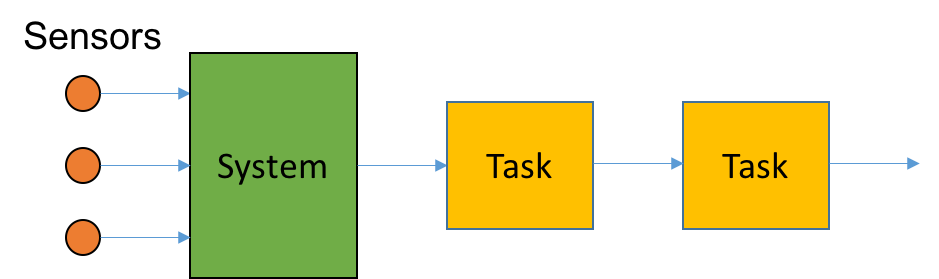
\includegraphics[width=0.8\textwidth]{includes/figures/fig_samza_overview}
  \caption{A simple Samza pipeline showing the roles of the system, task, and stream concepts. Streams are represented
  as arrows.}
  \label{fig:samza_overview}
\end{figure}

When programming a Samza project, interfaces exist for both the system and task concepts through the \texttt{org.apache.samza.system.SystemConsumer}
and \texttt{org.apache.samza.task.StreamTask} Java interfaces. Existing systems exist in the Samza project, and may be
used to produce streams which can then be processed by an implemented \texttt{StreamTask}.

The \texttt{StreamTask} interface is arguably the main interface in which the most important processing will be done in
a Samza project. It requires implementing a single method, \texttt{process}, which passes in an immutable message from the stream
on which the task is configured to consume. These messages are then processed as specified by the programmer before the
result of the processing is wrapped in a message envelope and produced to a stream specified by the programmer.

The streams on which \texttt{StreamTask} implementations consume are specified in a task specific configuration file,
independent to that of the implementation source code. These configuration files offer a range of parameters for the
execution of tasks, each of which are documented\footnote{https://samza.apache.org/learn/documentation/0.9/jobs/configuration-table.html},
however can result in quite verbose and hard to understand configurations files. For each task configuration, a system
needs to be defined that produces to the stream that the task consumes from. These can either be a self-implemented
system, or an existing pluggable system, such as Kafka.

For self-implementation of systems, then \texttt{SystemConsumer} interface requires much more understanding and effort to
implement than that of the \texttt{StreamTask} interface. Methods, such as \texttt{start}, \texttt{stop}, \texttt{register},
and \texttt{poll} need to be implemented, allowing for the producing of messages onto a particular stream. The \texttt{start}
and \texttt{stop} methods simply connect and disconnect the system to the underlying system, while the \texttt{poll}
method takes care of producing any messages from the system. The \texttt{register} method is much more complicated in the
way that it requires registering the implemented system with lower-level components of Samza to integrate the system into
Samza.

Note that, due to Samza's relative infancy to other DSPS technologies, many of these interfaces either completely lack
or offer insufficient documentation. Furthermore, for the same reason, example Samza projects are hard to find. This is
a key factor that will be touched upon in later chapters on evaluating the DSPS technologies.

Samza projects are generally compiled and distributed as JAR files, which may or may not contain project dependencies,
which then can be run directly on installed Samza distributions. Assembly of these JAR files are conventionally performed
through use of Java build automation tools, such as Maven or Gradle.

% subsubsection samza_programming (end)


\subsection{Storm Programming} % (fold)
\label{sub:storm_programming}

\textit{Note that most of the content in this section is sourced from the official Storm documentation.}~\cite{Storm:doc}

Storm defines itself as a distributed realtime computation system that provides primitives for performing realtime
computations. Storm compares itself to existing big data systems, such as Hadoop MapReduce, which similarly provides
primitives for performing batch data computations.

Like Samza, Storm also is built around the key concept of a stream, however Storm's definition of a stream slightly
differs to that of Samza's. In Storm, a stream is defined as an unbounded sequence of immutable tuples, rather than a sequence
of immutable messages as they are defined in Samza. A tuple is defined as a dynamically typed list of values, in which
the values can be of any type. Rather than consuming and producing to streams, Storm approaches computations on streams
through \textit{stream transformations} using the previously mentioned realtime computation primitives.

The realtime computation primitives that Storm offers are the components of Storm that are of most interest to the programmer.
These primitives are known as the \textbf{spout} and \textbf{bolt}, previously looked at in~\sectref{ssub:storm}. To compare
these components to those present in Samza, the spout acts as a source of streams, much like Samza's systems, while the
bolts acts as consumers of streams, which process and emit new streams, much like Samza's tasks. Storm offers interfaces
for implementation of custom spouts and bolts through the \texttt{backtype.storm.spout.ISpout} and \texttt{backtype.storm.task.IBolt}
interfaces, respectively.

As explained in~\sectref{ssub:storm}, spouts and bolts are arranged in a particular way to make up an overall Storm topology,
which is used to transform streams in some specified manner. A simple example of such a topology is shown in the previous
chapter, in~\figref{fig:storm_topology}.

Basic spouts require implementation of multiple methods, \texttt{open}, \texttt{nextTuple}, and \texttt{declareOutputFields},
which act as a spout initialiser, handler for each tuple to be emitted to a stream, and a tuple type declaration, respectively.
Implementation of a simple spout is a much easier task in Storm than a system in Samza, due to different provided interfaces
depending on the type of configuration needed for a particular spout. For example, a very basic spout can be made, using
a lot of default configuration options, by implementing the \texttt{backtype.storm.topology.base.BaseRichSpout} interface.

Bolts also require implementation of three main methods, \texttt{prepare}, \texttt{execute}, and \texttt{declareOutputFields},
allowing bolts to be initialised, process received tuples in a specified manner, and declare tuple value types, respectively.

One major point of different with this components, to their analogous components in Samza, is that the spout and bolt
implements are completely independent to the overall Storm topology layout. In Samza, systems and tasks require the output
streams to be hardcoded within their respective implementations, however Storm has a further separate source file for
defining the topology layout. This topology layout is generally defined in a separate file to all spout and bolt implementations
using the provided \texttt{backtype.storm.topology.ToplogyBuilder} class. This class exposes methods for defining the
topology layout, in terms of spout and bolt placement, along with inputs and outputs for each spout and bolt implementation,
as well as overall topology configuration. An obvious downside to this over Samza configuration files is that it requires
a recompilation in the case that configuration options need to be tweaked, while Samza configuration files are not part
of the compiled source code.

Storm topologies are generally compiled and distributed in the same way as Samza projects; as JAR files containing compiled
bytecode, assembled using Java build automation tools.

% subsection storm_programming (end)


\subsection{Spark Streaming Programming} % (fold)
\label{sub:spark_streaming_programming}

\textit{Note that most of the content in this section is sourced from the official Spark Streaming 1.3.1 documentation.}~\cite{Spark:doc}

While many analogies can be made between the key components of Storm and Samza, due to their similarities in design and
usage, Spark Streaming presents itself differently. Spark Streaming defines itself as an extension of its parent project,
Spark, a big data batch processing system, which affords scalable, high-throughput, fault-tolerant stream processing of
live data streams. Data can be streamed into Spark Streaming using a variety of supported sources, from complicated data
systems, such as Kafka, to low-level sources, such as TCP sockets.

Internally, Spark Streaming processes data quite differently to Samza and Storm, due to being an extension to the base
Spark batch processing system. Data streams are fed into Spark Streaming, which automatically partitions the streams into
small batches which are then sent to the underlying Spark batch processing engine. The Spark batch processing engine then
outputs a stream of results made up of multiple batches of data. A diagram illustrating this process is shown in~\figref{fig:spark_stream_batch}.

This way of processing streams as a sequence of batches is all enabled through Spark Streaming's stream abstraction,
discretised streams, or DStreams. It differs to how streams are conceptualised in Samza and Storm in the way that while
streams are still, in essence, an unbounded sequence of data structures, being tuples in Storm, and message envelopes in
Samza, these data structures are the same data structure which is used to represented data batches in Spark. These are,
of course, the same resilient distributed dataset (RDD) data structure as explained in the previous chapter, in~\sectref{ssub:spark_streaming}.
Hence, Spark Streaming DStreams can be decomposed into a sequence of RDDs, making them fully compatible with batch-mode Spark.

For programming a Spark Streaming job, there are not a set of provided interfaces expected to be implemented, like in
Samza or Storm. Instead, all of the computations to be performed on streams are performed on an instantiation of the
\texttt{org.apache.spark.streaming.dstream.DStream} class returned from a DStream producing function from the
\texttt{org.apache.spark.streaming.StreamingContext} class. Processing performed on DStreams are generally programmed in
a dataflow fashion, with each function performed on the DStream returning a new DStream.

This way of operating on DStreams in a Spark Streaming program leads to all processing being contained in a single file,
whereas in Storm or Samza processing would be split between tasks or bolts written in different files. This leads to
more straightforward control over DStream transformations when programming, however also leads to much more tightly
coupled logic. This will be a topic of interest later when evaluating the different DSPS technologies.

Spark Streaming programs are compiled and distributed in the same fashion in which Samza and Storm projects are. However,
for Spark Streaming programs written in Python using their relatively new PySpark API, compilation is unnecessary and an entire Spark
Streaming Python project can be distributed and submitted and run on different installations of Spark Streaming straight
from the Python source file. This greatly eases the distribution and deployment aspects of Spark Streaming, when using
PySpark, in relation to Storm topologies and Samza projects.

% subsection spark_streaming_programming (end)

% subsection dsps_technology_choices (end)



\subsection{Evaluation Method \& Approach} % (fold)
\label{sub:evaluation_method_approach}

Evaluation will be performed using both qualitative and quantitative methods. The quantitative evaluation methods used will focus
on the benchmarking of various features that are common to each of the technologies, and the comparison of the features that
each technology supports. The qualitative evaluation methods will focus on looking at the differences in ease-of-use,
support for different programming languages and features, and complexity of code written to implement the pipeline.

With looking at the decision of giving a clear recommendation for a particular technology out of the ones we have chosen,
we think it is import to look at both qualitative and quantitative aspects for comparison. These systems are significantly
non-trivial and vastly different in design and usage, however, as they still afford the same possible functionality,
it is very possible to give a properly constructed evaluation of them.


\subsubsection{Quantitative methods} % (fold)
\label{ssub:quantitative_methods}



% subsubsection quantitative_methods (end)


\subsubsection{Qualitative methods} % (fold)
\label{ssub:qualitative_methods}

The qualitative methods used to evaluate the DSPS systems for the pipeline will include the following:

\begin{itemize}
  \item
\end{itemize}

% subsubsection qualitative_methods (end)

% subsection evaluation_method_approach (end)



\subsection{Overview of the data} % (fold)
\label{sub:overview_of_the_data}

As this sub-project focuses on the realtime processing of streaming data, data streams will have to be simulated from
datasets acquired from the Monash IRT team. An initial dataset has been given that includes the following layout of data:

%TODO: table from my other paper

The sample data acquired from the IRT team includes 99\,999 rows of data recorded from each of the mentioned sensors,
organised in a CSV file with headers. This is a general example of how data is currently received and handled by the IRT
team, however in the case of realtime data processing, data would be received in quite a different manner. Rather than
being received in large batches of readings, such as the sample dataset acquired, streams of data may be created from
each particular sensor, delivering data values to the DSPS systems a single value at a time along those streams. Data
is streamed in an asynchronous fashion, and can be simply thought of as DSPS system listens on an incoming stream, and
acts upon any data value whenever they may be received.

Hence, to simulate streaming data from the data samples we have acquired, the DSPS pipeline is constructed to listen on
a particular socket connection for any incoming data. Once a data value is encountered on the connection, it is fed into
the pipeline and processed accordingly while the pipeline continues to listen on the socket for further incoming data.
As the pipeline is constructed in such a way, we can simulate the data being sent out from sensors using a program such
as \texttt{netcat}~\footnote{http://nc110.sourceforge.net/}, where we can pipe data from a file to a particular
socket over a connection.

% subsection overview_of_the_data (end)

\subsection{conclusion} % (fold)
\label{sub:conclusion}

% subsection conclusion (end)



% Section 4: Implementation
\section{Implementation}
\label{sec:implementation}
%!TEX root = thesis.tex
\chapter{Pipeline Design and Implementation}
\label{sec:implementation}

This chapter describes the design and implementation of the prototype data filtering pipelines to be built for testing
and evaluating our candidate data stream processing system (DSPS) technologies. This will be performed with the intention
of arriving at a recommendation system for the case study of the Monash University Institute of Railway Technology (IRT)
project. Each of the candidate DSPS technologies have been detailed in-depth in previous chapters, and all exhibit the capabilities
needed to implement the intended prototype pipelines.

This chapter will first go into the design of the data filtering pipeline, in~\sectref{sub:pipeline_design}, before
detailing the testing environment which was used to implement and test each pipeline, in~\sectref{sub:testing_environment_details}.
In~\sectref{sub:implementation_of_pipelines_in_dsps_technol}, the implementation of the prototype pipelines will be
detailed for each of the candidate DSPS technologies, as well as looking at the programming possibilities afforded by
each technology. Finally, the chapter will be concluded in~\sectref{sub:implement_conclusion}.


\section{Data Filtering Pipeline Design} % (fold)
\label{sub:pipeline_design}

The overall design of the data filtering pipeline will be designed in such a way that readings from sensors can be fed
into the pipeline, processed in some specified manner, then output for further use, including storage for batch processing,
or discarded in the case of noisy data. Thinking of the pipeline in such a way, we can decompose the design into three main
components:

\begin{enumerate}
  \item Sensor data input component
  \item Sensor data processing component
  \item Results output component
\end{enumerate}

Each component would also need to connect somehow to form the entire pipeline design. The components are listed
in order of their precedence of their role in the pipeline. Hence, the first component's output would be the input to
the second component, of which the output would be the input to the third component. This creates the dataflow behaviour
exhibited in pipelines. This basic design that we have so far is illustrated in~\figref{fig:pipeline_simple}.

\begin{figure}[ht]
  \centering
  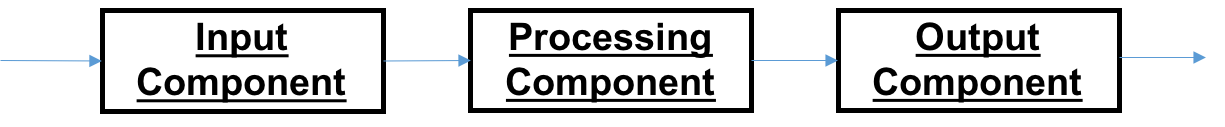
\includegraphics[width=0.8\textwidth]{includes/figures/fig_pipeline_simple}
  \caption{A simplistic overview of our pipeline design. Note the dataflow behaviour exhibited with each component's output
  being an input of the following component.}
  \label{fig:pipeline_simple}
\end{figure}

We now have a simple design of the pipeline, however we are left with the questions of the output of the \textbf{Output Component},
the input of the \textbf{Input Component}, and the contents of each component.

The output of the \textbf{Output Component}
will simply be whatever extensions are needed to be made to the pipeline. Hence, rather than acting a sink, this component
will be an abstract interface which any extension needed will be able to adhere to extend the pipeline. Designing the pipeline
in this manner directly addresses our third research question touched upon in Chapter 1, in~\sectref{sub:research_questions}.
This allows the output data to be dealt with in any manner required by the IRT team, whether it be stored for later
batch processing, or forwarded on for further realtime processing.

The input of the \textbf{Input Component} will be the data read from the sensors to which the pipeline is connected to.
The sensors generally would not be directly connected to the pipeline, so we could have another abstract interface here
that any sensor connects to, then the interface sends the data to the actual component. This allows data to be fed into
the pipeline from any type of sensor that is able to adhere to the interface.

The contents of each component is a larger task. The \textbf{Processing Component} will be made up
of an arbitrary number of tasks, each of which are tasked to process the data in some manner before forwarding it onto whatever
the next specified task is. This, in itself, acts as a mini-pipeline where the core of processing will be done. Here
we will say that the \textbf{Processing Component} consists of $n$ sequential processing tasks. For the \textbf{Input Component},
the contents will consist of a task-like component tasked with passing data onto the processing tasks which make up the
\textbf{Processing Component}. The contents of the
\textbf{Output Component} will be as described previously: an abstract interface allowing for the extension of the pipeline.

This leaves us with a final pipeline design as illustrated in~\figref{fig:pipeline_whole}.

\begin{figure}[ht]
  \centering
  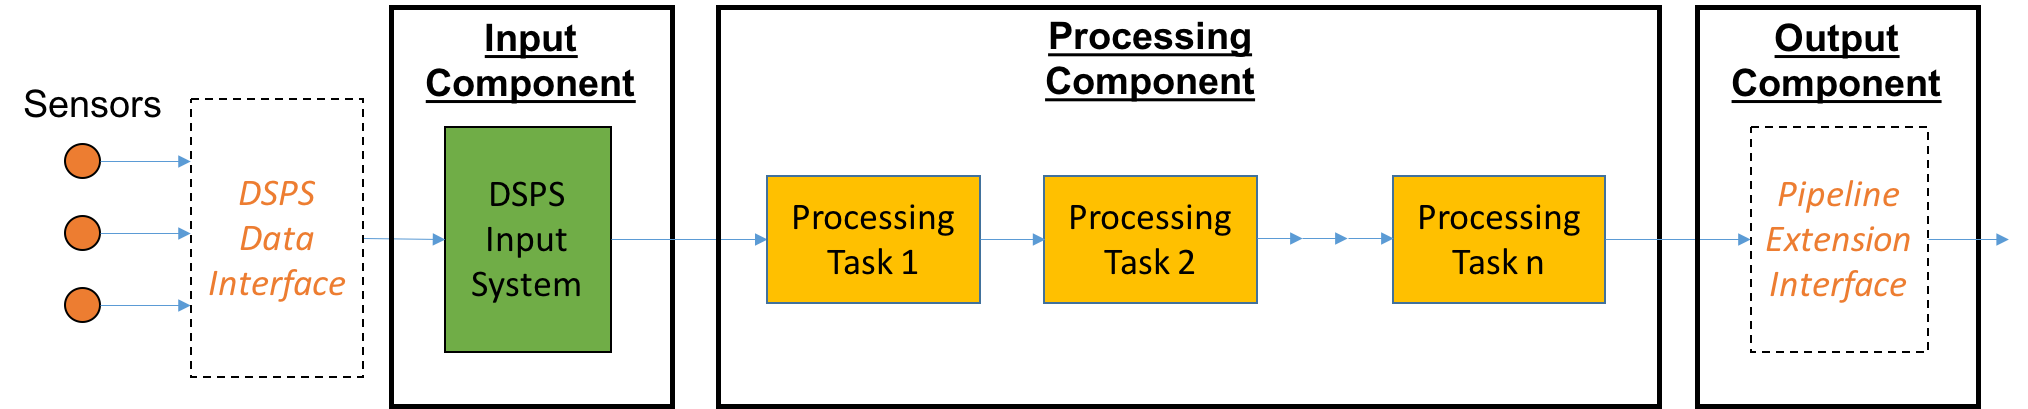
\includegraphics[width=1\textwidth]{includes/figures/fig_pipeline_whole}
  \caption{A complete overview of our pipeline design.}
  \label{fig:pipeline_whole}
\end{figure}

Note that this diagram illustrates an overall abstract pipeline design. However, for implementation of the pipeline which
will be used in the evaluation parts of the project, we need to implement concrete components for testing. In this project,
we do not have access to any sensors, or any such hardware, for sending readings to the pipeline for processing. Hence, for evaluation
we have had to simulate the sensor component of the overall pipeline design in some way. Note that this does not affect
the pipeline in any way, since the actual sensor hardware part of the design is abstracted away from the software pipeline
itself. The function of the sensors is to send data to the pipeline at any arbitrarily specified interval through use of the
DSPS Data Interface.
To simulate this functionality multiple methods exist. The most basic of such is arguably reading data from a file
and placing that onto a stream for the pipeline to process. However, this very much mimics batch processing methods, and
hence is not ideal for simulating realtime data. Furthermore, placing data from a file onto the pipeline does not accurately
reflect the client-server networking functionality that will exist in a real sensor-pipeline connection.

A better way to simulate this sensor-pipeline realtime data connection is to develop a data entry interface to the pipeline upon which data can be sent to
at any time. This data entry interface can then be used to simulate arbitrarily specified intervals upon which data can be sent,
thus mimicking the functionality of a sensor. To do this while still adhering to the client-server connection design,
we can use a socket connection, allowing data to be sent over a specified port to be placed upon the pipeline. Each
candidate DSPS technology either has native support for server socket connections, given their commonplace as mediums upon
which data can be sent over, or support from the programming language standard libraries used to implement realtime processing logic.

Hence, the \textbf{Input Component} will be implemented as a server socket connection,
and the \textbf{Processing Component} as a filtering task. Speed sensor readings will be passed in along the socket connection
using a tool allowing interface to network ports, such as \texttt{netcat}\footnote{http://netcat.sourceforge.net/}, and filtered to make sure they are valid
speed values, between the limits of 0 and 90. Any speeds
outside of these limits can safely be deemed to be either bad, or noisy, sensor readings. This results in a concrete design as shown
in~\figref{fig:pipeline_concrete}.

\begin{figure}[ht]
  \centering
  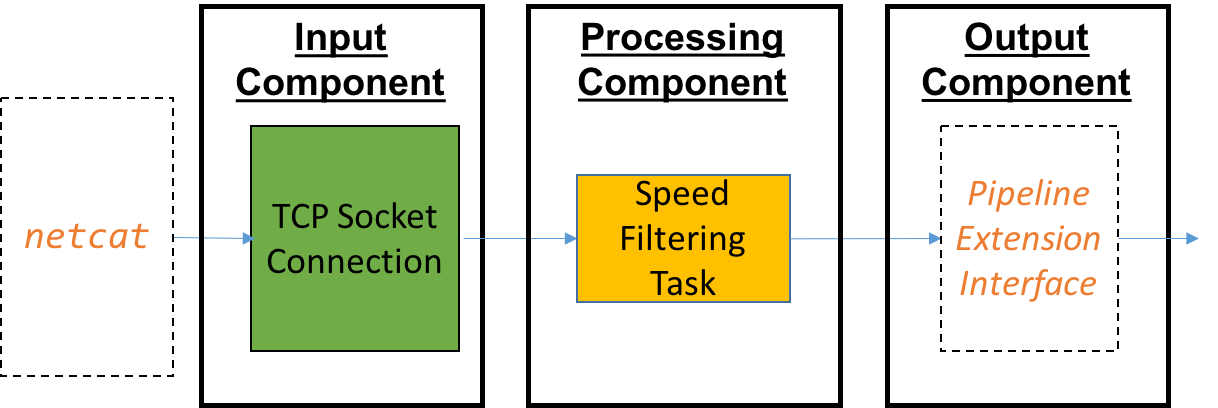
\includegraphics[width=0.8\textwidth]{includes/figures/fig_pipeline_concrete}
  \caption{A concrete implementation of our pipeline design.}
  \label{fig:pipeline_concrete}
\end{figure}

% subsection pipeline_design (end)


\section{Testing Environment Details} % (fold)
\label{sub:testing_environment_details}

\subsection{Details on Host System} % (fold)
\label{ssub:host_system}

The testing environment on which the prototype pipelines were implemented using each of the candidate DSPS technologies
is the same National eResearch Collaboration Tools and Resources (NeCTAR) cloud computing environment touched upon
briefly in Chapter 1. This cloud service platform is provided as an initiative by the Australian Government for researchers
that require the infrastructure\footnote{https://www.nectar.org.au/about-nectar}.

Our environment consists of a single NeCTAR cloud instance of which the details are specified in~\tabref{tab:control}.

\begin{table}[ht]
\caption{Control system used for testing pipelines.}
\label{tab:control}
\centering
\begin{tabular}{ll}
\textbf{Distribution}         & Ubuntu GNU/Linux 14.04.2 LTS \\
\textbf{Kernel}               & Linux 3.13.0-36-generic    \\
\textbf{Architecture}         & x86\_64                    \\
\textbf{Virtual CPUs}         & 16                         \\
\textbf{Available RAM}        & 64 GB                      \\
\textbf{Available Disk Space} & 490 GB
\end{tabular}
\end{table}

The NeCTAR cloud instance utilises a single node upon which all processing is performed. In a real deployment, it is
common to use a full cluster upon which the pipeline would be deployed, where processing is shared and distributed between nodes. Due to
limited testing resources, all testing
has been performed on a single node cluster, however this remains a constant feature between all implementation and tests
performed in the project. Furthermore, the pipelines built upon
each of the candidate DSPS technologies are freely configurable to be deployed to run on arbitrarily sized clusters without
requiring changes to the underlying source code.

% subsubsection host_system (end)


\subsection{Details on Data Stream Processing System Technologies} % (fold)
\label{sub:setting_up_of_dsps_technologies}

The DSPS technologies that have been chosen to be focused on in this sub-project include the following:

\begin{itemize}
  \item Samza
  \item Storm
  \item Spark Streaming
\end{itemize}

Literature concerning these DSPS technologies have been covered in~\sectref{sub:realtime_data_processing}, however
we will look into more depth into the systems regarding their usage from the programmer's point-of-view. Note that
in the previous chapter, a further DSPS technology, S4, was covered, however due to its noted decline in usage and
development in the chapter, it has been decided to omit the use of the technology from this project.

Version 0.9.0 of Samza was used for implementation of the prototype pipeline in Samza. At the time of implementation,
this was the major stable version of Samza, accepted as a top-level Apache project. Java, the only official programming
language supported by the Samza project, was used, using JDK 1.8.0 as the target implementation.

Version 0.9.4 of Storm was used for implementation of the prototype pipeline in Storm. As with Samza, this was also the
major stable version of Storm available. Java 8 was used as the implementation language, also compiling for the JDK 1.8.0.

Version 1.3.0 of Spark and the Spark Streaming extension were used for the Spark Streaming implementations. Prototype pipelines were
implemented in both Scala 2.9.2, targeting the JDK 1.8.0, and Python 2.7, which is made possible through the relatively new (as of Spark 1.2.0)
PySpark subsystem. Implementations for the Spark Streaming pipeline were built targeting both Spark JVM and PySpark due
to numerous undocumented claims that performance differs on both Spark implementations. These claims are addressed further
in the following chapter.

The specific JDK implementation for all tests was the Intel 64-bit OpenJDK 1.8.0 release 45 built and packaged for the GNU/Linux
distribution of Ubuntu 14.04.2 LTS.

% subsubsection setting_up_of_dsps_technologies (end)

% subsection testing_environment_details (end)


\section{Implementation of Pipelines in Data Stream Processing System Technologies} % (fold)
\label{sub:implementation_of_pipelines_in_dsps_technol}

Here, we will look at how the each of the candidate DSPS technologies were used for implementation in relation to our testing
pipeline design. We will look at the possibilities each technology affords in terms of programmability, and then what was
required to be implemented for our testing and evaluation to arrive at a DSPS recommendation.

For each DSPS technology, we will look at what was needed to be implemented for the following components from our design:

\begin{itemize}
  \item Input component
  \item Processing component
  \item Output component
\end{itemize}

\subsection{Samza} % (fold)
\label{ssub:impl_samza}

Samza defines itself as a realtime data processing system, which allows the processing of streams made up of immutable
messages of similar type or category. Streams in Samza exist independently of other concepts, allowing themselves to be
\textit{consumed} from or \textit{produced} to by various supported systems. The concepts of consuming and producing refer
to the actions of getting data from a stream and placing data onto a stream, respectively. Samza defines the systems that can be used
for consuming and producing to streams to be any piece of software that implements the stream abstraction. For example,
Kafka, a popular distributed messaging queueing system, is often used to consume and produce to Samza streams. Systems such as these can be
``plugged'' into a Samza project to work with the same streams which native Samza applications are written to work with~\cite{Samza:doc}.

For a Samza programmer, the most important concepts of the overall Samza project to understand are the concepts of the
\textbf{system} and \textbf{task}. In a Samza project, a system exists to produce a particular stream from some source
of data which then can
be processed by a task which consumes it. A task will always perform some processing before producing the results as output to another stream. Systems and tasks
can then be arranged in a pipeline-like structure allowing a specified type of processing on the messages which travel
on those streams. Hence, it is easy to think of a system as the source of data for an overall Samza project. A very
simple example of such a Samza project is shown in~\figref{fig:samza_overview}.

\begin{figure}[ht]
  \centering
  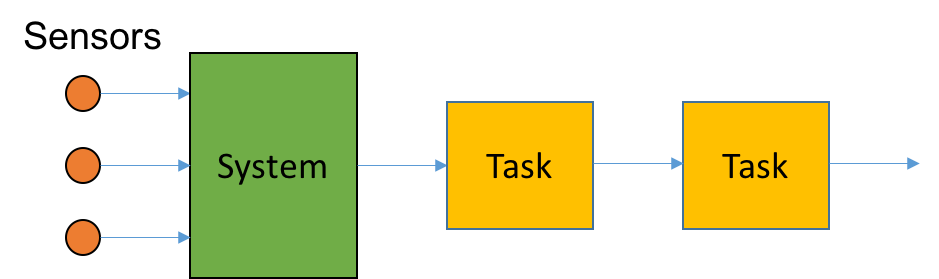
\includegraphics[width=0.8\textwidth]{includes/figures/fig_samza_overview}
  \caption{A simple Samza pipeline showing the roles of the system (handling input data), task (handling data processing), and stream concepts. Streams are represented
  as arrows.}
  \label{fig:samza_overview}
\end{figure}

\subsubsection{Programming Overview}

When programming a Samza project, interfaces exist for both the system and task concepts through the \path{org.apache.samza.system.SystemConsumer}
and \path{org.apache.samza.task.StreamTask} Java interfaces~\cite{Samza:doc}. Default systems exist in the Samza project, and may be
used to produce streams which can then be processed by an implemented \texttt{StreamTask}.

The \texttt{StreamTask} interface is arguably the main interface in which the most important processing will be done in
a Samza project. It requires implementing a single method, \texttt{process}, which passes in an immutable message from the stream
on which the task is configured to consume. These messages are then processed as specified by the programmer, before the
result of the processing is wrapped in a message envelope and produced to a stream, also specified by the programmer~\cite{Samza:doc}.

The streams on which \texttt{StreamTask} implementations consume are specified in a task specific configuration file,
independent to that of the implementation source code. These configuration files offer a range of parameters for the
execution of tasks, each of which are documented\footnote{https://samza.apache.org/learn/documentation/0.9/jobs/configuration-table.html},
however can result in quite verbose and hard to understand configuration files. For each task configuration, a system
needs to be defined that produces to the stream that the task consumes from. These can either be a self-implemented
system, or an existing pluggable system, such as Kafka~\cite{Samza:doc}.

For self-implementation of systems, the \texttt{SystemConsumer} interface requires much more understanding and effort to
implement than that of the \texttt{StreamTask} interface. Methods, such as \texttt{start}, \texttt{stop}, \texttt{register},
and \texttt{poll} need to be implemented, allowing for the producing of messages onto a particular stream. The \texttt{start}
and \texttt{stop} methods simply connect and disconnect the system to the underlying system, while the \texttt{poll}
method takes care of producing any messages from the system. The \texttt{register} method is much more complicated in the
way that it requires registering the implemented system with lower-level components of Samza to integrate the system into
Samza~\cite{Samza:doc}.

Note that, due to Samza's relative infancy, compared with other DSPS technologies, many of these interfaces either completely lack
or offer insufficient documentation. Furthermore, for the same reason, example Samza projects are hard to find. This is
a key factor that will be touched upon in the next chapter on evaluating the DSPS technologies.

\subsubsection{Input Component}

For implementation of the input component design in Samza, this revolves around the \texttt{SystemConsumer} interface.
As we want the Samza system to produce to a stream based on values received over a server socket connection, we can use
an instantiation of the \path{java.net.ServerSocket} class to do this. This can be set up in the system's constructor
and then, in the system's \texttt{start} method, attempt to poll any incoming values using a \path{java.io.InputStream} generated
from that connection. If any values are encountered on that connection, we can produce them to the default speed value
stream, which will consumed by the filtering task.

The system's \texttt{stop} method simply will be used to close the server connection, while the \texttt{register} method will
be used to register the system with the previously mentioned default speed value stream.

\subsubsection{Processing Component}

For the implementation of the processing component design in Samza, this revolves around the \texttt{StreamTask} interface.
This Samza task will get its input by consuming from the same stream on which the previously detailed Samza system implementation
produced to. The main \texttt{process} method can then be used to consume a value from the stream, then check if the value
received is between the acceptable speed limits. Depending on the outcome of this test, the message is either flagged for
being noisy, or not, and then produced to a stream for valid values, or a stream for noisy data. This allows the filtering
of data, with flagged data being produced to a separate stream to those data that are deemed to be valid.

\subsubsection{Output Component}

For the output component of our designed pipeline, no implementation needs to be done. Samza, by design, affords extension
by implementing a new \texttt{StreamTask} that is configured to consume from an existing stream in the Samza project.

\subsubsection{Deployment}

Samza projects are generally compiled and distributed as JAR files, which may or may not contain project dependencies,
which then can be run directly on installed Samza distributions. Assembly of these JAR files are conventionally performed
through use of Java build automation tools, such as Maven or Gradle.

For the implementation of our designed pipeline, Maven was used to assemble a JAR file containing compiled bytecode, which can be deployed on different
Samza installations.

\textit{Note that the source code of our implementation can be seen in Appendix~\ref{lst:samza}.}

% subsubsection samza (end)


\subsection{Storm} % (fold)
\label{ssub:impl_storm}

Storm defines itself as a distributed realtime computation system that provides primitives for performing realtime
computations. Storm compares itself to existing big data systems, such as Hadoop MapReduce, which similarly provides
primitives for performing batch data computations.

Like Samza, Storm also is built around the key concept of a stream, however Storm's definition of a stream slightly
differs to that of Samza's. In Storm, a stream is defined as an unbounded sequence of immutable tuples, rather than a sequence
of immutable messages as they are defined in Samza. A tuple is defined as a dynamically typed list of values, in which
the values can be of any type. Rather than consuming and producing to streams, Storm approaches computations on streams
through \textit{stream transformations} using the previously mentioned realtime computation primitives.

\subsubsection{Programming Overview}

The realtime computation primitives that Storm offers are the components of Storm that are of most interest to the programmer.
These primitives are known as the \textbf{spout} and \textbf{bolt}, previously looked at in~\sectref{ssub:storm}. To compare
these components to those present in Samza, the spout acts as a source of streams, much like Samza's systems, while the
bolts act as consumers of streams, which process and emit new streams, much like Samza's tasks. Storm offers interfaces
for implementation of custom spouts and bolts through the \path{backtype.storm.spout.ISpout} and \path{backtype.storm.task.IBolt}
interfaces, respectively~\cite{storm_doc}.

As explained in~\sectref{ssub:storm}, spouts and bolts are arranged in a particular way to make up an overall Storm topology,
which is used to transform streams in some specified manner. A simple example of such a topology is shown in the previous
chapter, in~\figref{fig:storm_topology}.

Basic spouts require implementation of multiple methods, \texttt{open}, \texttt{nextTuple}, and \texttt{declareOutputFields},
which act as a spout initialiser, handler for each tuple to be emitted to a stream, and a tuple type declaration, respectively.
Implementation of a simple spout is a much easier task in Storm than a system in Samza, due to different provided interfaces
depending on the type of configuration needed for a particular spout. For example, a very basic spout can be made, using
a lot of default configuration options, by implementing the \path{backtype.storm.topology.base.BaseRichSpout} interface~\cite{storm_doc}.

Bolts also require implementation of three main methods, \texttt{prepare}, \texttt{execute}, and \texttt{declareOutputFields},
allowing bolts to be initialised, process received tuples in a specified manner, and declare tuple value types, respectively~\cite{storm_doc}.

One major point of difference with these components, relative to their analogous components in Samza, is that the spout and bolt
implements are completely independent to the overall Storm topology layout. In Samza, systems and tasks require the output
streams to be hardcoded within their respective implementations, however Storm has a further separate source file for
defining the topology layout. This topology layout is generally defined in a separate file to all spout and bolt implementations
using the provided \path{backtype.storm.topology.ToplogyBuilder} class. This class exposes methods for defining the
topology layout, in terms of spout and bolt placement, along with inputs and outputs for each spout and bolt implementation,
as well as overall topology configuration~\cite{storm_doc}. An obvious downside to this over Samza configuration files is that it requires
a recompilation in the case that configuration options need to be tweaked, while Samza configuration files are not part
of the compiled source code.

\subsubsection{Input Component}

For the implementation of the input component design in Storm, this revolves around the \texttt{BaseRichSpout} interface.
Much like the Samza implementation, this implementation also uses \path{java.net.ServerSocket} and \path{java.io.InputStream}
for listening on a server socket connection for incoming speed values. The \texttt{open} method is used for the creation
of such a server socket connection, while the \texttt{nextTuple} method is used for attempted to read any values off the
connection. If a value is encountered, it is constructed into a Storm tuple containing the speed value, and emitted onto
the configured stream. The \texttt{declareOutputFields} method is then used to declare the speed value type as a single
value of type Double to be expected to make up a valid tuple.

\subsubsection{Processing Component}

For the implementation of the processing component design in Storm, this revolves around the \texttt{BaseRichBolt} interface.
The \texttt{execute} method is used to test the data value in the received tuple in the same way as tested in the Samza
implementation. Based on the outcome of the test, a new tuple is made with two values: the speed value along with a
noise flag, being flagged if the speed value fails the test, unflagged otherwise. The newly constructed tuple is then
emitted to the output stream for further processing.

\subsubsection{Output Component}

As with the Samza implementation, the Storm implementation of the designed pipeline does not require any concrete implementation
of the output component. This is as Storm, by design, allows any extension to be made to a topology simply by implementing
a further bolt which receives its tuples from an existing stream.

\subsubsection{Deployment}

Storm topologies are generally compiled and distributed in the same way as Samza projects; as JAR files containing compiled
bytecode, assembled using Java build automation tools.

For the implementation of our designed pipeline, Maven was used to assemble a JAR file containing compiled bytecode, which
is free to be deployed on different Storm installations.

\textit{Note that the source code of our implementation can be seen in Appendix~\ref{lst:storm}.}

% subsubsection storm (end)


\subsection{Spark Streaming} % (fold)
\label{ssub:impl_spark_streaming}

For Spark Streaming, we have implemented the designed pipeline in both Python and Scala, running on the PySpark and Spark
JVM systems, respectively. However, as the programming interface is mostly the same between both projects, the two
implementations remain sufficiently similar, apart from being written in two different programming languages, that it is
not needed to write about them separately. For parts of the implementation that differ between the two systems, they
will be noted.

While many analogies can be made between the key components of Storm and Samza, due to the two project's similarities in design and
usage, Spark Streaming presents itself differently. Spark Streaming defines itself as an extension of its parent project,
Spark, a big data batch processing system, which affords scalable, high-throughput, fault-tolerant stream processing of
live data streams. Data can be streamed into Spark Streaming using a variety of supported sources, from complicated data
systems, such as Kafka, to low-level sources, such as server sockets.

\subsubsection{Programming Overview}

Internally, Spark Streaming processes data quite differently to Samza and Storm, due to being an extension to the base
Spark batch processing engine. Data streams are fed into Spark Streaming, which automatically partitions the streams into
small batches which are then sent to the underlying Spark batch processing engine. The Spark batch processing engine then
outputs a stream of results made up of multiple batches of data. A diagram illustrating this process is shown in~\figref{fig:spark_stream_batch}.

\begin{figure}[H]
  \centering
  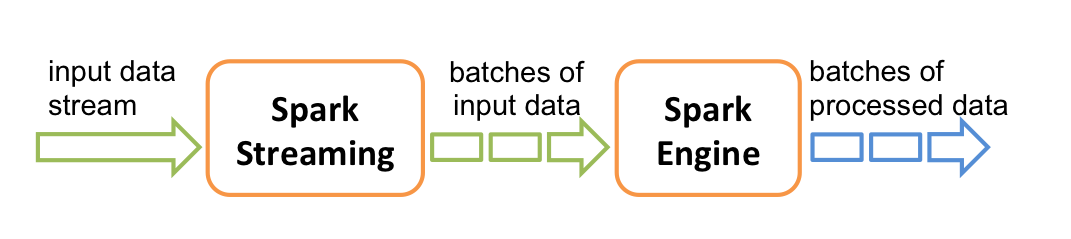
\includegraphics[width=0.8\textwidth]{includes/figures/fig_spark_layout}
  \caption{Illustration~\cite{Spark_doc_fig} depicting how Spark Streaming runs on-top of the Spark batch engine.}
  \label{fig:spark_stream_batch}
\end{figure}

This way of processing streams as a sequence of batches is all enabled through Spark Streaming's stream abstraction,
discretised streams, or DStreams. It differs to how streams are conceptualised in Samza and Storm in the way that while
streams are still, in essence, an unbounded sequence of data structures, being tuples in Storm, and message envelopes in
Samza, these data structures are the same data structure which is used to represented data batches in Spark. These are,
of course, the same resilient distributed dataset (RDD) data structure as explained in the previous chapter, in~\sectref{ssub:spark_streaming}.
Hence, Spark Streaming DStreams can be decomposed into a sequence of RDDs, making them fully compatible with batch-mode Spark~\cite{spark_stream_doc}.

For programming a Spark Streaming job, there are not a set of provided interfaces expected to be implemented, like in
Samza or Storm. Instead, all of the computations to be performed on streams are performed on an instantiation of the
\path{org.apache.spark.streaming.dstream.DStream} class returned from a DStream producing function from the
\path{org.apache.spark.streaming.StreamingContext} class~\cite{spark_stream_doc}. Processing performed on DStreams are generally programmed in
a dataflow fashion, with each function performed on the DStream returning a new DStream.

This way of operating on DStreams in a Spark Streaming program leads to all processing being contained in a single file,
whereas in Storm or Samza processing would be split between tasks or bolts written in different files. This leads to
more straightforward control over DStream transformations when programming, however also leads to much more tightly
coupled logic. This will be a topic of interest later when evaluating the different DSPS technologies.

\subsubsection{Input Component}

For the implementation of the input component design in Spark Streaming, Spark Streaming provides a native server socket input
system built-in on the \texttt{StreamingContext} class, available through the \texttt{socketTextStream} method. Hence
this has been used to open a connection on a particular server socket for inputting of speed data in the same manner as in the
Samza and Storm implementations.

\subsubsection{Processing Component}

For the implementation of the processing component design in Spark Streaming, a function has been written to test a single
speed value, testing whether or not it is between the specified speed limits. Depending on the outcome of the test,
a tuple is returned containing the original speed value, and a noise flag that is flagged if the data value is outside
of the speed limit.

This speed test function then gets mapped to the existing socket connection DStream, effectively running the function
for every speed value that is received over the connection.

\subsubsection{Output Component}

Unlike the Storm or Samza implementations, Spark Streaming offers no simple way to extend an existing streaming processing
project through means of extra processing tasks that operate on existing streams. However, it does afford extensibility
in the way of adding further processing on the DStream that is produced from previously performed operations, such
as the previously mentioned speed test function mapping.

\subsubsection{Deployment}

Spark Streaming programs are compiled and distributed in the same fashion in which Samza and Storm projects are. However,
for Spark Streaming programs written in Python using their relatively new PySpark API, compilation is unnecessary and an entire Spark
Streaming Python project can be distributed and submitted and run on different installations of Spark Streaming straight
from the Python source file. This greatly eases the distribution and deployment aspects of Spark Streaming, when using
PySpark, in relation to Storm topologies and Samza projects.

For our Spark Streaming pipeline implementation written in Scala, SBT\footnote{http://www.scala-sbt.org/} was used to assemble a JAR file containing compiled
bytecode, for ease of use over Maven with Scala projects. For the Spark Streaming pipeline implemented in Python, the
Python source files were simply used for deployment. Both methods enable the deployment of the Spark Streaming pipelines on
different Spark installations.

\textit{Note that the source code of our implementation can be seen in Appendix~\ref{lst:spark}.}

% subsubsection spark_streaming (end)




\section{Conclusion} % (fold)
\label{sub:implement_conclusion}

In conclusion this chapter has touched upon all details of implementation for each of the prototype pipelines.
We have detailed how each prototype data filtering pipeline has been built for each candidate system, ready
for subsequent tests and evaluation, of which will be discussed in the following chapter. Furthermore, the overall
design of the pipeline that has been implemented has been detailed along with the details of the overall testing
environment upon which the pipelines are to be implemented.

% subsection conclusion (end)


% Section 5: Evaluation
\section{Discussion and Evaluation}
\label{sec:evaluation}
%!TEX root = thesis.tex
\section{Discussion and Evaluation}
\label{sec:evaluation}

In order to evaluate the three different data stream processing system technologies used to build the proposed pipeline,
we compare them in terms of both quantitative and qualitative measures. The quantitative measures used to contrast
each technology include aspects such as start-up time, data response time, data throughput allowance, and system resource
usage. The qualitative measures used the contrast each technology will highlight different aspects such as ease-of-programmability,
available features, ease-of-deployment, and ease-of-extensibility. Each of these measures will be expanded on in
both~\sectref{sub:quantitative_evaluations} and~\sectref{seb:qualitative_evaluations}.

The control for each of the evaluation measures will be the system on which the different technologies are deployed.
Each identically-functioning pipeline built using different DSPS technologies will be deployed in the same NeCTAR cloud
instance, as highlighted in%TODO: section reference
The control NeCTAR cloud instance system is touched upon further in~\sectref{sub:testing_environment}.

This chapter begins with an overview of the NeCTAR testing environment, in~\sectref{sub:testing_environment}, upon which
all tests are performed. Quantitative evaluations and results are then described in~\sectref{sub:quantitative_evaluations},
while qualitative evaluations and results are described in~\sectref{sub:qualitative_evaluations}. Discussion of the
evaluations and subsequent DSPS technology recommendations will be given in~\sectref{sub:dsps_technology_recommendations},
before concluding in~\sectref{sub:conclusion}.


\subsection{Testing environment} % (fold)
\label{sub:testing_environment}

The testing environment upon which all needed tests will be performed also acts as the major control constant between
each of the different DSPS systems that have been built. The environment is based on a single NeCTAR cloud instance, as detailed
in%TODO: sectref to nectar stuff
. The system details of the given instance are detailed in~\tabref{tab:control}.

\begin{table}[h]
\caption{Control system used for testing pipelines.}
\label{tab:control}
\centering
\begin{tabular}{ll}
\textbf{Distribution}         & Ubuntu GNU/Linux 14.04.2 LTS \\
\textbf{Kernel}               & Linux 3.13.0-36-generic    \\
\textbf{Architecture}         & x86\_64                    \\
\textbf{Virtual CPUs}         & 16                         \\
\textbf{Available RAM}        & 64 GB                      \\
\textbf{Available Disk Space} & 490 GB
\end{tabular}
\end{table}

The NeCTAR cloud instance utilises a single node upon which all processing is performed. In a real deployment, it is
common to use a full cluster upon which the pipeline would be deployed, where processing is shared between nodes. Due to
limited testing resources, all testing
has been performed on a single node cluster, however this is still a constant feature between all tests, and the pipelines built upon
each of the existing technologies are freely configurable to be deployed to run on arbitrarily sized clusters without
needing changes to the underlying source code.

% subsection testing_environment (end)


\subsection{Quantitative Evaluations} % (fold)
\label{sub:quantitative_evaluations}

\subsubsection{Testing data} % (fold)
\label{ssub:testing_data}

The testing data for the quantitative stage of evaluation includes data sourced from actual readings from the speed
sensors attached to train cars in the Monash University Institute of Railway Technology data project. We use a total
of 99\,999 discrete speed readings, some of which are altered to give bad values. The base function of
the built pipelines is to detect bad, or noisy, values and flag them before forwarding all values on for further processing
in the pipeline, as explained in~\sectref{sec:implementation}. This is an example of actual realtime data processing that
the Monash IRT team have indicated they would be interested in performing.

Hence, the test data is all known. The majority of the test data readings are valid speed readings, however the pipelines
built will detect all those which are not valid and flag them.

% subsubsection testing_data (end)


\subsubsection{Tests to be performed} % (fold)
\label{ssub:tests_to_be_performed}

The quantitative tests to be performed and contrasted will include the following:

\begin{itemize}
  \item System start-up time
  \item Response time to streaming data
  \item Data throughput allowance
  \item System resource usage
\end{itemize}

Each of these can be quantified and compared easily via tracking various aspects of the system.

Start-up time will
be measured from the time each DSPS technology is started via the system shell until the time the DSPS technology is
ready to accept incoming data streams. This can be measured using the UNIX \texttt{time} command, and allowing the
DSPS technology terminate upon start-up, as well as the timestamps recorded in the output logs for each of the DSPS
technologies.

Response time will be measured by the amount of time a ready DSPS technology takes from the time a data value is pushed
onto the input stream until the time that the result of that given data value is pushed onto the output stream. This
can be measured using the output logs for each of the DSPS technologies.

Data throughput allowance will be measured by comparing how much time it takes for the DSPS technology to process the
entirety of our test data. This can be measured using the output logs for each of the DSPS technologies.

System resource usage will be measured by comparing the amount of system memory \textit{reserved} for use for each
of the running DSPS technologies. These are expected to vary during runtime, so samples will be taken at the peak system
resource usage of each DSPS technology during the processing of our test data.
Measurements will be taken using the UNIX tool
\texttt{ps} to collect readings for the amount of CPU usage and virtual memory reserved for use by the DSPS technology.
Note that the amount of memory reported by \texttt{ps} is simply the amount of virtual memory reserved for use by the
process, as opposed to the actual amount of memory being used.

% subsubsection tests_to_be_performed (end)


\subsubsection{Outcomes of Tests Performed} % (fold)
\label{sub:outcomes_of_tests_performed}



% subsection outcomes_of_tests_performed (end)

% subsection quantitative_evaluations (end)


\subsection{Qualitative Evaluations} % (fold)
\label{sub:qualitative_evaluations}


\subsection{Tests to be performed} % (fold)
\label{sub:tests_to_be_performed}

The qualitative tests to be performed and contrasted will include the following:

\begin{itemize}
  \item Ease of programmability
  \item Available DSPS features
  \item Ease of deployment
  \item Ease of extensibility
\end{itemize}

As each of the underlying systems are considerably different in

% subsection tests_to_be_performed (end)

% subsection qualitative_evaluations (end)


\subsection{DSPS Technology Recommendations} % (fold)
\label{sub:dsps_technology_recommendations}

% subsection dsps_technology_recommendations (end)



% Section 6: Conclusion
\section{Conclusions}
\label{sec:conclusion}
%!TEX root = thesis.tex



% Bibliography
\bibliographystyle{acm}
\bibliography{thesis.bib}

\end{document}
